\documentclass{beamer}
\usepackage{beamerthemeshadow}
\usepackage[utf8x]{inputenc}
\begin{document}
\title{Hackerspace Prague}
\author{brmlab}
\date{\today}

\frame{
\begin{figure}
   
\includegraphics{logo.pdf}
\end{figure}
}

\frame{\frametitle{Co je hackerspace?}
\begin{itemize}
\item prostor, kde lidé sdílejí společné zájmy - vědu, technologie, digitální nebo elektronické umění a dokážou se učit nad rámec své školy či práce
\item otevřená, vysoce kreativní komunita
\item koncentrace mladé technologické elity
\item nekomerční, nezisková a nezávislá organizace
\end{itemize}
}

\frame{\frametitle{Funkce hackerspace}
\begin{itemize}
\item centrum vzdělávání a výměny zkušeností
\item pracovní skupiny organizující pravidelné workshopy, prezentace nebo odborné přednášky
\item prostor pro tvorbu komunitních i individuálních projektů
\item základní infrastruktura pro členy
  \begin{itemize}
  \item síťové připojení, projektory, 3D tiskárny, unikátní hardware a software, elektrotechnické a dílenské vybavení
  \end{itemize}
\end{itemize}
}

\frame{\frametitle{Proč hackerspace v Praze?}
\begin{itemize}
\item koncentrace a socializace lidí s podobnými zájmy
\item možnost kooperace na zajímavých komunitních a veřejně-prospěšných projektech
\item přístup k zajímavým (pro jednotlivce drahým) nejnovějším technologiím
\item přínos v informatizaci společnosti díky otevřenosti hackerspace pro veřejnost
\item podpora mladých talentů a výchova podnikavé technologické elity
\item spolupráce s existujícími vědeckými institucemi a univerzitami
\end{itemize}
}

\frame{\frametitle{Právní forma}
\begin{itemize}
\item nekomerční, nezisková, plně otevřená, transparentní a nezávislá organizace
\item občanské sdružení na demokratické bázi
\end{itemize}
}

\frame{\frametitle{Příjmy hackerspace}
\begin{itemize}
\item členské příspěvky
  \begin{itemize}
  \item vzhledem na požadovanou nezávislost by mělo být co nejvíce základních výdajů pokryto z těchto příspěvků
  \end{itemize}
\item granty
\item sponzorské dary
\end{itemize}
}

\frame{\frametitle{Členství}
\begin{itemize}
\item po zaplacení členského příspěvku
  \begin{itemize}
  \item 500 Kč / 20 EUR měsíčně
  \item studenti 50%% sleva
  \end{itemize}
\item umožňuje přístup do hackerspace, možnost využívat veškeré jeho technické vybavení, infrastrukturu a jiné prostředky
\end{itemize}
}

\frame{\frametitle{Pracovní skupiny}
\begin{itemize}
\item vedené zkušenými profesionály v dané oblasti
\item organizace pravidelných setkání
\item otevřené a dostupné všem členům hackerspace
\item revoluční vzdělávací přístup
  \begin{itemize}
  \item rovnocenná pozice učitele i žáka - učitel se stává studentem, student učitelem
  \end{itemize}
\end{itemize}
}

\frame{\frametitle{Projekty}
\begin{itemize}
\item počítačový software a hardware
\item elektronika a robotika
\item augmentovaná a virtuální realita
\item digitální umění, audio/video laboratoř
\item informační bezpečnost
\item místo pro události
\end{itemize}
}

\frame{\frametitle{Existujíci hackerspace}
\begin{itemize}
\item na celém světe je jich víc než 500
\item 62! v Německu, 5 v Rakousku
\item Metalab Vídeň
\item HSPBP Budapešť
\item ProgressBar Bratislava
\end{itemize}
}

\frame{\frametitle{Metalab Vídeň}
\begin{itemize}
\item více než 200 m$^{2}$ v centru Vídně
\item více než 100 platících členů
\item výrazná finanční pomoc od města Vídeň
\item sponzorské příspěvky
\item možnost realizace finančně náročných projektů
\end{itemize}
}

\frame{\frametitle{Metalab Vídeň}
\begin{figure}
   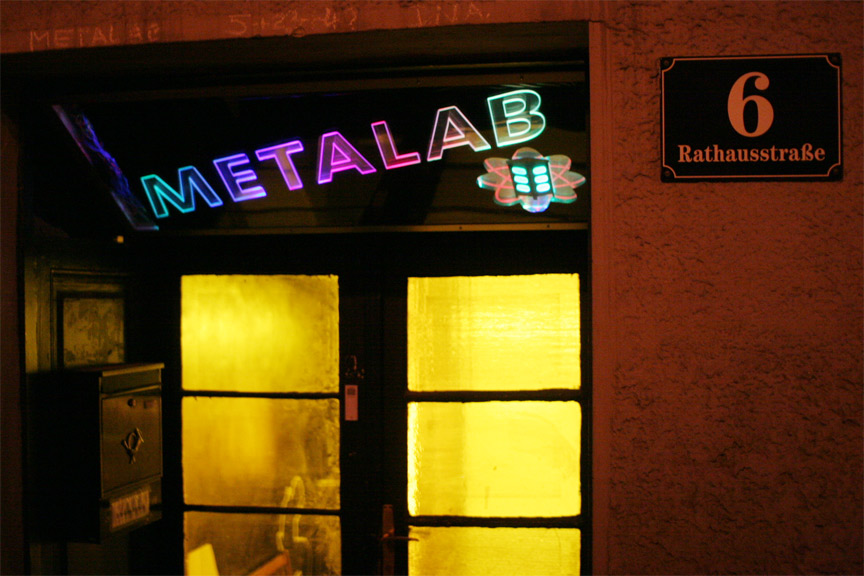
\includegraphics[width=10.5cm,height=7cm,bb=0 0 864 576]{metalab1.jpg}
\end{figure}
}

\frame{\frametitle{Metalab Vídeň}
\begin{figure}
   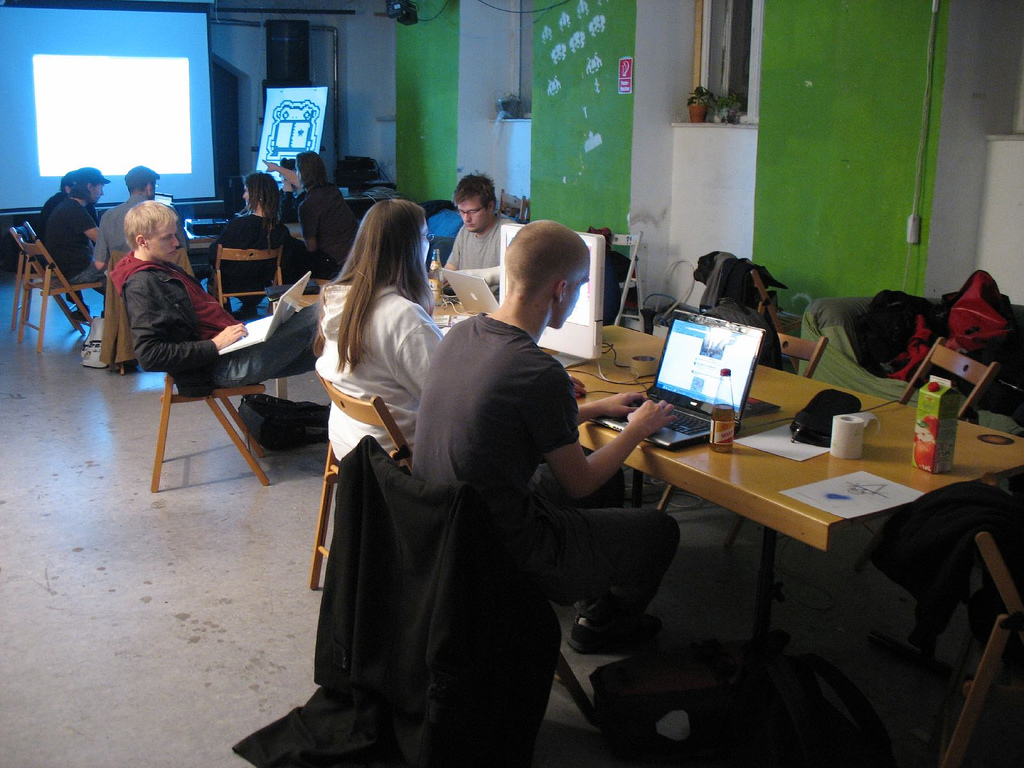
\includegraphics[width=9.33cm,height=7cm,bb=0 0 1024 768]{metalab2.jpg}
\end{figure}
}

\frame{\frametitle{Metalab Vídeň}
\begin{figure}
   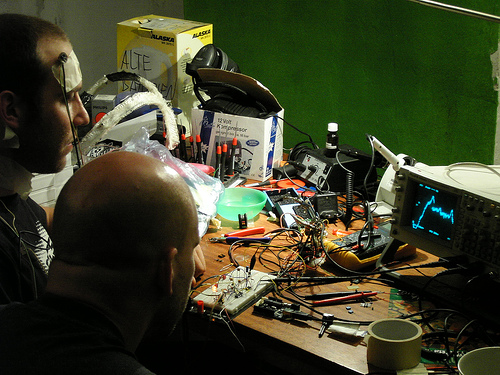
\includegraphics[width=9.33cm,height=7cm,bb=0 0 500 375]{metalab3.jpg}
\end{figure}
}

\frame{\frametitle{Metalab Vídeň}
\begin{figure}
   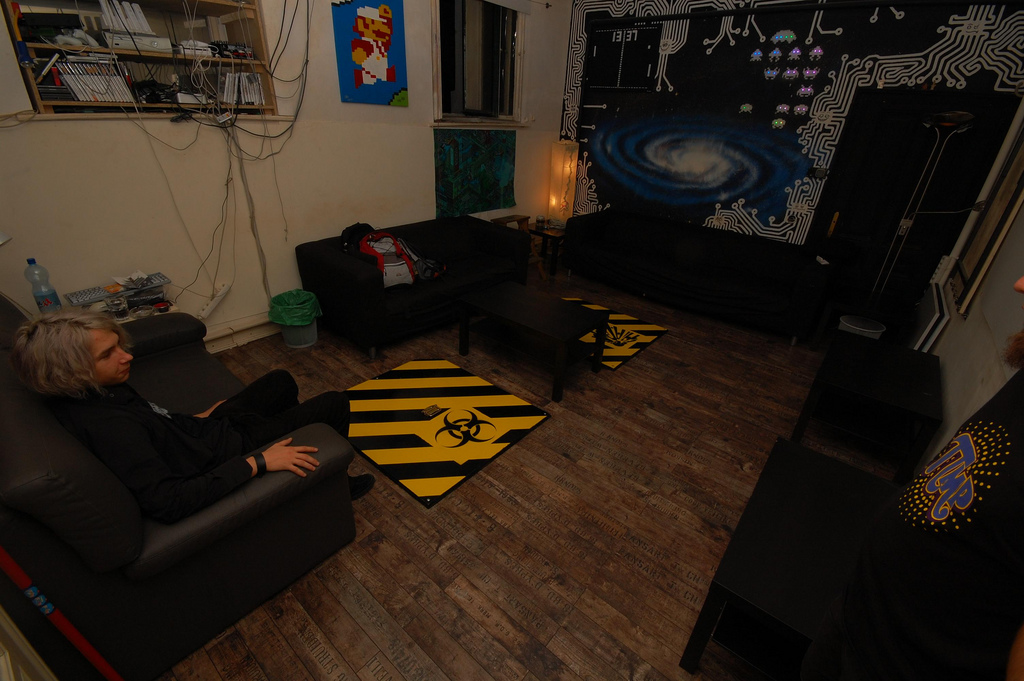
\includegraphics[width=10.5cm,height=7cm,bb=0 0 1024 681]{metalab4.jpg}
\end{figure}
}

\frame{\frametitle{Metalab Vídeň}
\begin{figure}
   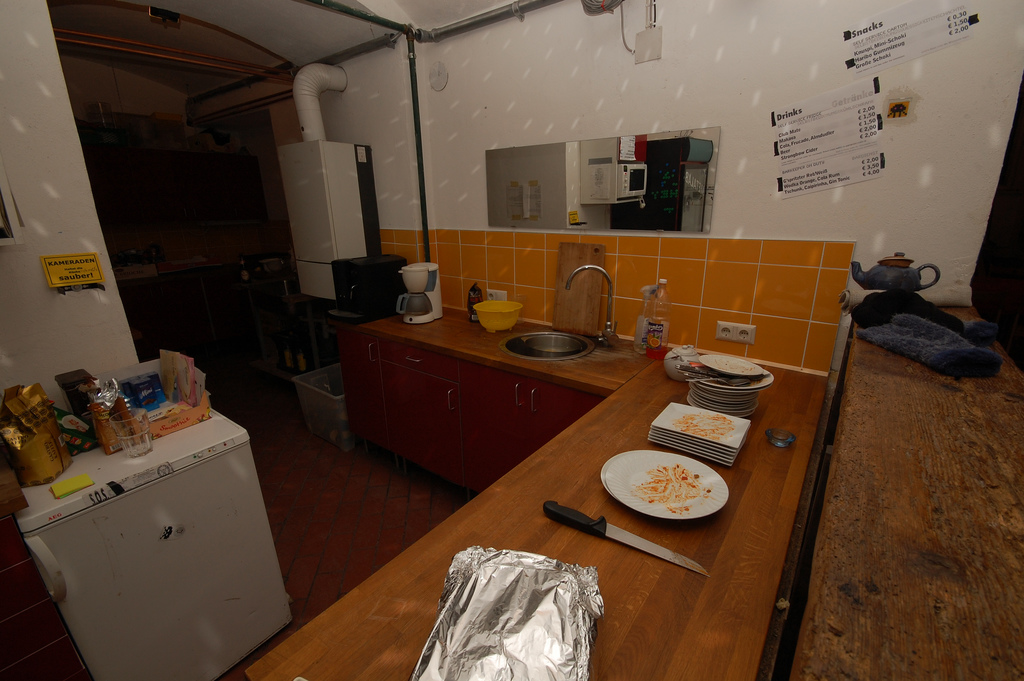
\includegraphics[width=10.5cm,height=7cm,bb=0 0 1024 681]{metalab5.jpg}
\end{figure}
}

\frame{\frametitle{Status}
\begin{itemize}
\item občanské sdružení
  \begin{itemize}
  \item momentálně 20 členů
  \item dedikované bankové účty
  \end{itemize}
\item infrastruktura
  \begin{itemize}
  \item web: brmlab.cz
  \item mailing list: brmlab@brmlab.cz
  \item IRC: \#brmlab@freenode
  \end{itemize}
\item prostory
  \begin{itemize}
  \item Kamenická 13
  \end{itemize}
\end{itemize}
}

\frame{\frametitle{Aktivity}
\begin{itemize}
\item Brmbot Outdoor
\item Brmbot Turing
\item Mitch Altman workshop
\item ...
\end{itemize}
}

\frame{\frametitle{Brmbot Outdoor}
\begin{figure}
   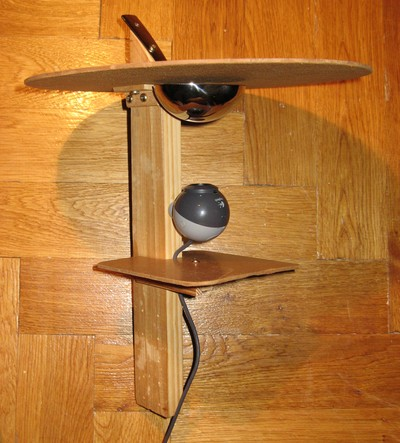
\includegraphics[width=6.32cm,height=7cm,bb=0 0 400 443]{brmcam_mk_i.jpg}
\end{figure}
}

\frame{\frametitle{Brmbot Outdoor}
\begin{figure}
   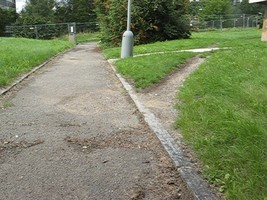
\includegraphics[width=9.345cm,height=7cm,bb=0 0 267 200]{brm_improc_tst.jpg}
\end{figure}
}

\frame{\frametitle{Brmbot Outdoor}
\begin{figure}
   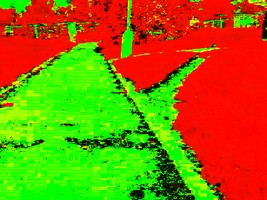
\includegraphics[width=9.345cm,height=7cm,bb=0 0 267 200]{brm_improc_tst_hsv_filt.jpg}
\end{figure}
}

\frame{\frametitle{Brmbot Outdoor}
\begin{figure}
   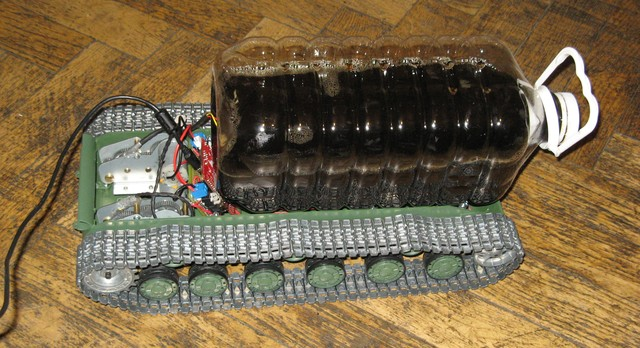
\includegraphics[width=10cm,height=5.4375cm,bb=0 0 640 348]{brmchassis.jpg}
\end{figure}
}

\frame{\frametitle{Brmbot Turing}
\begin{figure}
   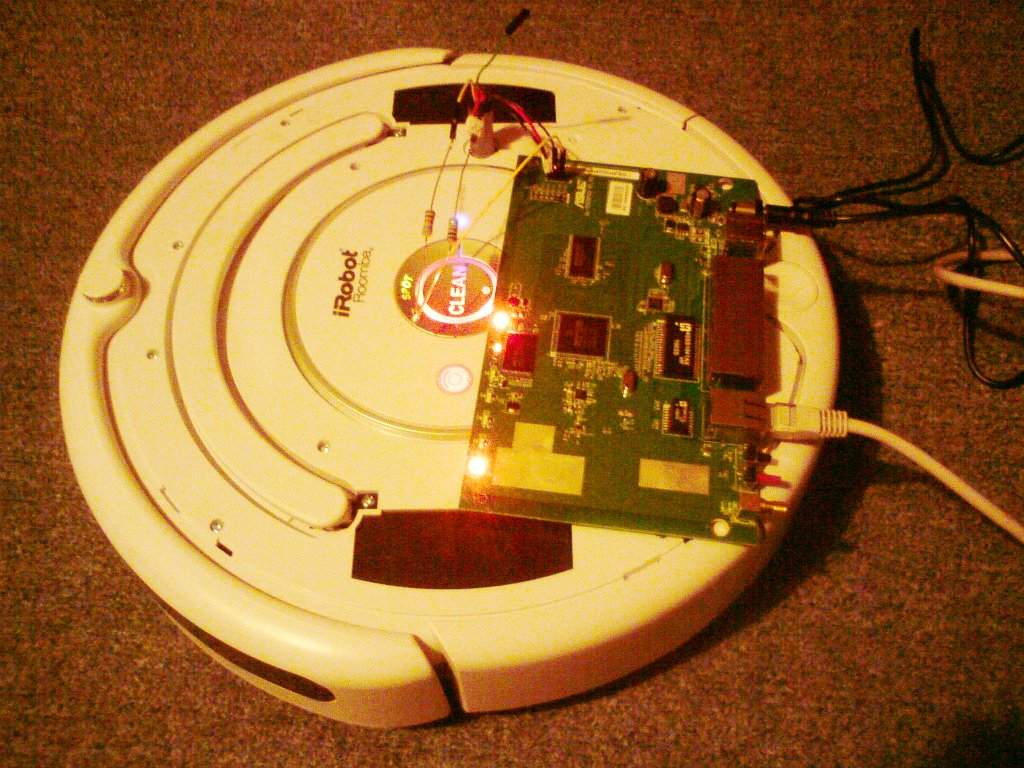
\includegraphics[width=9.33cm,height=7cm,bb=0 0 1024 768]{roomba_asus.jpg}
\end{figure}
}

\frame{\frametitle{Mitch Altman workshop}
\begin{figure}
   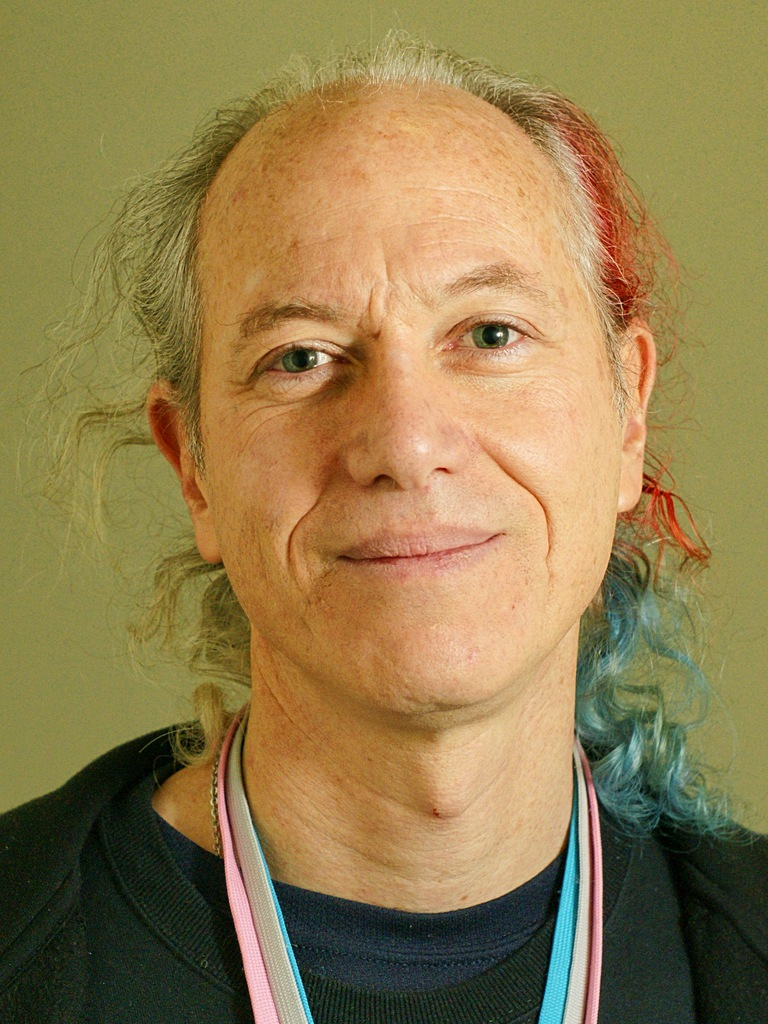
\includegraphics[width=5.25cm,height=7cm,bb=0 0 768 1024]{altman.jpg}
\end{figure}
}

\frame{\frametitle{Mitch Altman workshop}
\begin{figure}
   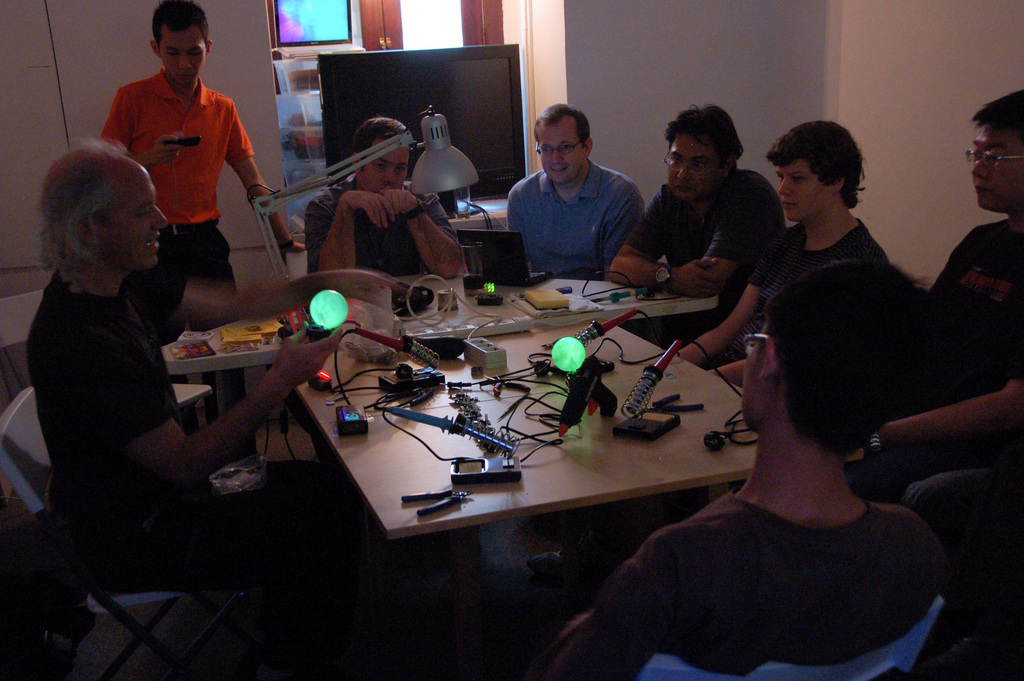
\includegraphics[width=10.5cm,height=7cm,bb=0 0 1024 681]{altman-workshop.jpg}
\end{figure}
}

\end{document}
